\chapter{EDA Lab III: Will a Data Scientist Change Jobs? (Real HR Data)}
\companion{pandas User Guide: Working with missing data}{https://pandas.pydata.org/docs/user_guide/missing_data.html}

This chapter uses a \textbf{real} dataset from your repository, \code{Data\_gathering/dataset/aug\_train.csv} (Kaggle ``HR Analytics: Job Change of Data
Scientists''): 19{,}158 candidates who took a company's data-science training, with profile, education, current company, experience and training hours; the target is 1 if the
candidate is looking for a new job. It is a near-perfect stand-in for Naukri data, and it is messy in exactly the ways real job-portal data are. Notebook section: \emph{Case 2}.
All outputs are from real runs.

\section{Step 1: load, overview, target}
\begin{lstlisting}
hr = load_csv("Data_gathering/dataset/aug_train.csv"); print(hr.shape)
overview(hr)
hr["target"].value_counts(normalize=True)
\end{lstlisting}
\outlabel
\begin{lstlisting}[style=out]
(19158, 14)
                          dtype  missing  missing_%  n_unique                  example
enrollee_id               int64        0        0.0     19158                     8949
city                        str        0        0.0       123                 city_103
city_development_index  float64        0        0.0        93                     0.92
gender                      str     4508       23.5         3                     Male
relevent_experience         str        0        0.0         2  Has relevent experience
enrolled_university         str      386        2.0         3            no_enrollment
education_level             str      460        2.4         5                 Graduate
major_discipline            str     2813       14.7         6                     STEM
experience                  str       65        0.3        22                      >20
company_size                str     5938       31.0         8                    50-99
company_type                str     6140       32.0         6                  Pvt Ltd
last_new_job                str      423        2.2         6                        1
training_hours            int64        0        0.0       241                       36
target                  float64        0        0.0         2                      1.0
target: 0.0 -> 0.751, 1.0 -> 0.249
\end{lstlisting}
\textbf{Say}: ``One row per candidate; 25\% are looking to change: imbalanced, so PR AUC and F1, stratified splits, maybe class weights. Two numeric columns only; experience and
last-new-job are numbers stored as text; city has 123 levels; company fields are a third missing.''

\section{Step 2: types and data quality}
\begin{lstlisting}
for c in ["experience", "last_new_job", "company_size"]:
    print(c, hr[c].value_counts(dropna=False).to_dict())
\end{lstlisting}
\outlabel
\begin{lstlisting}[style=out]
experience: {'>20': 3286, '5': 1430, '4': 1403, ..., '1': 549, '<1': 522, ..., '20': 148, nan: 65}
last_new_job: {'1': 8040, '>4': 3290, '2': 2900, 'never': 2452, '4': 1029, '3': 1024, nan: 423}
company_size: {nan: 5938, '50-99': 3083, '100-500': 2571, '10000+': 2019, '10/49': 1471,
               '1000-4999': 1328, '<10': 1308, '500-999': 877, '5000-9999': 563}
\end{lstlisting}
Three issues an interviewer wants you to spot: (1) \code{experience} is ordinal text with codes \code{>20} and \code{<1}; (2) \code{last\_new\_job} has \code{>4} and \code{never}; (3)
\code{company\_size} has a malformed label \code{10/49} (every other band uses a hyphen, so it should be \code{10-49}). Also notice \code{>20} is the single most common experience value:
a capped variable (we cannot distinguish 21 from 35 years).
\begin{lstlisting}
hr["experience_num"] = hr["experience"].replace({">20": "21", "<1": "0"}).astype(float)
hr["last_new_job_num"] = hr["last_new_job"].replace({">4": "5", "never": "0"}).astype(float)
hr["company_size"] = hr["company_size"].replace({"10/49": "10-49"})
size_order = ["<10", "10-49", "50-99", "100-500", "500-999", "1000-4999", "5000-9999", "10000+"]
hr["company_size_ord"] = hr["company_size"].map({s: i for i, s in enumerate(size_order)})
print("duplicates ignoring id:", hr.drop(columns="enrollee_id").duplicated().sum())    # 49
\end{lstlisting}
\code{company\_size} is ordinal, so an \textbf{ordinal map} keeps the order (0--7) instead of one-hot. The 49 duplicates (identical except ID) are 0.26\% of rows: note and keep,
or deduplicate if they are re-registrations.

\section{Step 3: missing values, with the target}
\begin{lstlisting}
missing_vs_target(hr[["gender", "enrolled_university", "education_level", "major_discipline", "experience",
                      "company_size", "company_type", "last_new_job", "target"]], "target")
\end{lstlisting}
\outlabel
\begin{lstlisting}[style=out]
             column  missing_%  target_rate_if_missing  target_rate_if_present
       company_type       32.0                   0.388                   0.184
       company_size       31.0                   0.406                   0.179
             gender       23.5                   0.308                   0.231
   major_discipline       14.7                   0.195                   0.259
    education_level        2.4                   0.226                   0.250
       last_new_job        2.2                   0.364                   0.247
enrolled_university        2.0                   0.319                   0.248
         experience        0.3                   0.354                   0.249
\end{lstlisting}
\begin{center}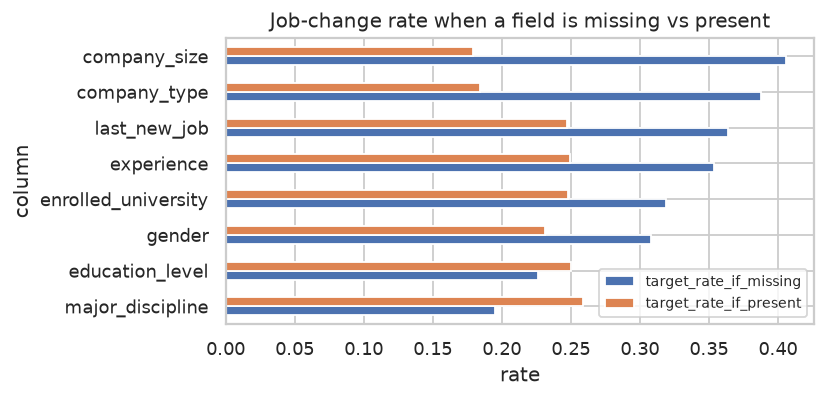
\includegraphics[width=0.65\linewidth]{eda_lab/figs/hr_missing_vs_target.png}\end{center}
\textbf{Reading}:
\begin{itemize}
\item When company size or type is blank, the job-change rate is about \textbf{40\%} versus about \textbf{18\%} when present: more than double. Combined with the fact that they are
  missing \emph{together} (Chapter 41, R4), the likely meaning is ``not currently employed'', a strong reason to look for a job. This is \textbf{informative missingness}
  (not MCAR).
\item Missing gender also carries a higher rate (31\% vs 23\%): people who skip optional fields may be less engaged or different.
\item Missing major discipline goes the other way (20\% vs 26\%): probably candidates without a degree.
\end{itemize}
\textbf{Decisions}: never drop these rows (53\% of rows have something missing); encode the missingness of company size, company type and gender as an explicit \code{"Unknown"}
level (or a missing indicator); for GBMs leave NaN; do not impute company size with the mode (that would erase the 40\% signal).

\section{Step 4: numeric features}
\begin{lstlisting}
num_summary(hr[["city_development_index", "training_hours", "experience_num", "last_new_job_num"]])
\end{lstlisting}
\outlabel
\begin{lstlisting}[style=out]
                          count   mean    std   min    25%   50%    75%     max  skew  kurt  n_iqr_outliers  n_zeros
city_development_index  19158.0   0.83   0.12  0.45   0.74   0.9   0.92    0.95 -1.00 -0.54              17        0
training_hours          19158.0  65.37  60.06  1.00  23.00  47.0  88.00  336.00  1.82  3.84             984        0
experience_num          19093.0  10.10   6.78  0.00   4.00   9.0  16.00   21.00  0.41 -1.17               0      522
last_new_job_num        18735.0   2.00   1.68  0.00   1.00   1.0   3.00    5.00  0.80 -0.76               0     2452
\end{lstlisting}
\begin{center}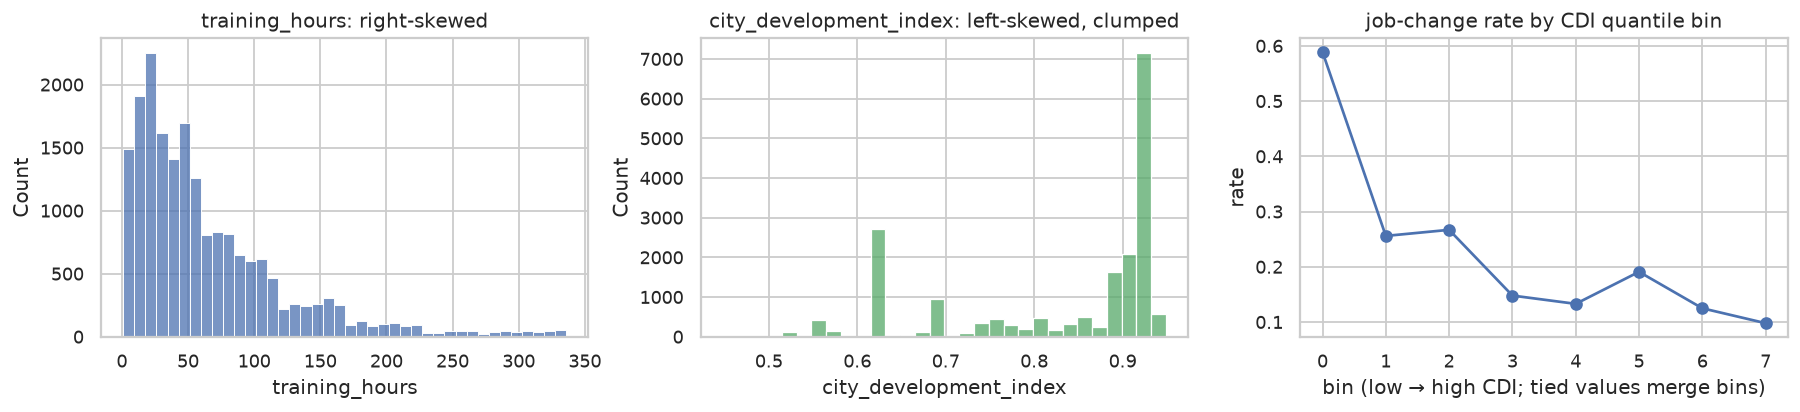
\includegraphics[width=\linewidth]{eda_lab/figs/hr_numeric.png}\end{center}
\begin{lstlisting}
rate_by(hr, "city_development_index", "target", q=5)
point_biserial(hr, ["city_development_index", "training_hours", "experience_num", "last_new_job_num"], "target")
\end{lstlisting}
\outlabel
\begin{lstlisting}[style=out]
                         rate     n                         feature   r_pb  p_value
(0.447, 0.691]          0.551  3869          city_development_index -0.342    0.000
(0.691, 0.878]          0.206  3827                  experience_num -0.177    0.000
(0.878, 0.92]           0.178  8925                last_new_job_num -0.083    0.000
(0.92, 0.949]           0.104  2537                  training_hours -0.022    0.003
\end{lstlisting}
\textbf{Reading}:
\begin{itemize}
\item \textbf{City development index (CDI)} is left-skewed and \emph{clumped} (only 93 distinct values: it is a city-level number shared by everyone in a city). It is the strongest
  numeric signal and strongly \textbf{non-linear}: 55\% of candidates in the least developed cities want to move, against 10--21\% elsewhere; the drop happens almost entirely at the
  bottom. A linear model will under-fit this; use bins, a spline, or a tree model.
\item \textbf{training\_hours} is right-skewed (skew 1.8, 984 IQR ``outliers'' that are genuine heavy learners) and almost unrelated to the target ($r = -0.02$; flat across
  quartiles in R16). The $p = 0.003$ is ``significant'' only because $n$ is huge: statistically detectable, practically useless.
\item Experience: more experience, less job change ($r = -0.18$); 522 candidates with $<$1 year.
\end{itemize}

\section{Step 5: categorical features}
\begin{lstlisting}
for c in ["relevent_experience", "enrolled_university", "education_level", "company_type", "last_new_job"]:
    print(rate_by(hr, c, "target").sort_values("rate", ascending=False))
\end{lstlisting}
\outlabel
\begin{lstlisting}[style=out]
relevent_experience   No 0.338 (5366) | Has 0.215 (13792)
enrolled_university   Full time 0.381 (3757) | MISSING 0.319 (386) | Part time 0.252 (1198) | none 0.211 (13817)
education_level       Graduate 0.280 | MISSING 0.226 | Masters 0.214 | High School 0.195 | Phd 0.140 | Primary 0.133
company_type          MISSING 0.388 (6140) | Other 0.240 | Early Stage Startup 0.235 | Public Sector 0.220
                      | NGO 0.186 | Pvt Ltd 0.181 (9817) | Funded Startup 0.140 (1001)
last_new_job          MISSING 0.364 | never 0.301 | 1 0.264 | 2 0.241 | 3 0.226 | 4 0.222 | >4 0.182
\end{lstlisting}
\begin{lstlisting}
[(c, cramers_v(hr[c].fillna("MISSING"), hr["target"])) for c in [...]]
\end{lstlisting}
\begin{center}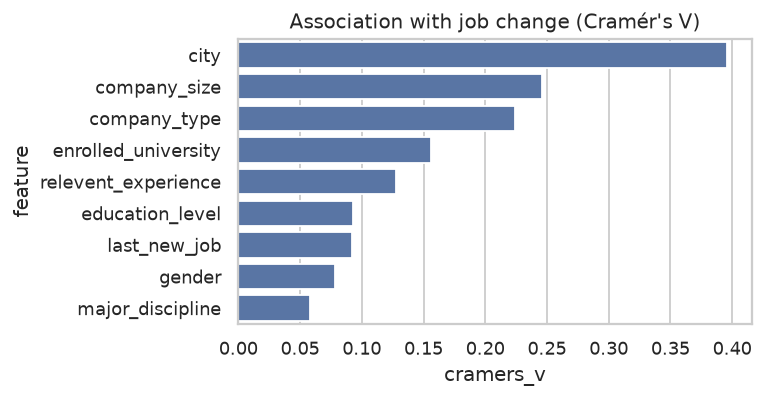
\includegraphics[width=0.6\linewidth]{eda_lab/figs/hr_cramers.png}\end{center}
\outlabel
\begin{lstlisting}[style=out]
city 0.396 | company_size 0.246 | company_type 0.224 | enrolled_university 0.156 | relevent_experience 0.128
education_level 0.093 | last_new_job 0.092 | gender 0.078 | major_discipline 0.058
\end{lstlisting}
\textbf{Reading}: city is the strongest categorical feature; company size and type are next, \emph{mostly because of their MISSING level}; full-time students (38\%) and people without
relevant experience (34\%) are the most likely to move; employees of funded startups the least (14\%). \code{last\_new\_job} shows a monotone pattern: the longer since the last job
change, the less likely to change now.

\section{Step 6: the high-cardinality city}
\begin{lstlisting}
cs = hr.groupby("city").agg(n=("target", "size"), rate=("target", "mean"), cdi=("city_development_index", "first"))
print("cities:", len(cs), "| cities with < 20 candidates:", (cs["n"] < 20).sum())
print("CDI constant within each city?", (hr.groupby("city")["city_development_index"].nunique() == 1).all())
print("corr(city rate, city CDI) =", round(cs["rate"].corr(cs["cdi"]), 3))
prior, m = hr["target"].mean(), 20
cs["smoothed_rate"] = (cs["n"] * cs["rate"] + m * prior) / (cs["n"] + m)
\end{lstlisting}
\outlabel
\begin{lstlisting}[style=out]
cities: 123 | cities with < 20 candidates: 44
CDI constant within each city? True
corr(city rate, city CDI) = -0.705
             n   rate    cdi  smoothed_rate
city_103  4355  0.213  0.920          0.213
city_21   2702  0.591  0.624          0.589
city_16   1533  0.117  0.910          0.118
city_114  1336  0.100  0.926          0.102
\end{lstlisting}
\textbf{Reading}: 44 of 123 cities have fewer than 20 candidates, so their raw rates are noise; one-hot would add 122 sparse columns. CDI is a \emph{property of the city} and explains much of
the city effect (correlation $-0.71$ between a city's rate and its CDI). One city alone, \code{city\_21} (CDI 0.624, 2{,}702 candidates, 59\% movers), drives a large share of the
low-CDI signal: a business question in itself. \textbf{Encoding plan}: keep CDI; add city frequency; add out-of-fold \textbf{smoothed target encoding} (shown with $m = 20$);
group rare cities.

\section{Step 7: experience and an interaction}
\begin{lstlisting}
hr.groupby(pd.cut(hr["experience_num"], [-1, 2, 5, 10, 15, 21]))["target"].agg(["mean", "size"])
sns.pointplot(data=hr, x=pd.cut(hr["experience_num"], [-1, 2, 5, 10, 15, 21]).astype(str), y="target",
              hue="relevent_experience", errorbar=None)
\end{lstlisting}
\outlabel
\begin{lstlisting}[style=out]
(-1, 2]   0.384  2198      (2, 5]   0.322  4187      (5, 10]  0.252  5011
(10, 15]  0.191  2829      (15, 21] 0.156  4868
\end{lstlisting}
\begin{center}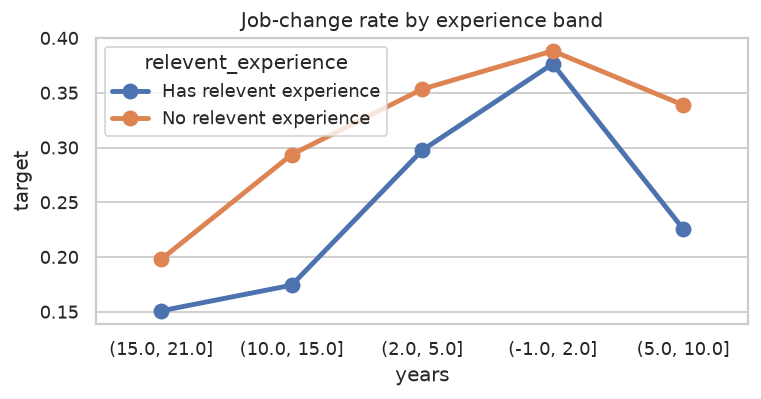
\includegraphics[width=0.6\linewidth]{eda_lab/figs/hr_experience.png}\end{center}
\textbf{Reading}: job-change propensity falls steadily with experience (38\% for 0--2 years to 16\% for 15+). At every experience level, candidates without relevant experience are
more likely to move: they are trying to switch into data science.

\section{Step 8: findings and the modelling plan}
\begin{enumerate}
\item 19{,}158 candidates, 25\% movers: imbalanced; use stratified CV, PR AUC/F1, class weights; threshold by recruiter capacity.
\item Fix types: parse \code{experience} and \code{last\_new\_job} (note the cap at 20+), repair the \code{10/49} label, ordinal-encode company size; drop \code{enrollee\_id}.
\item \textbf{Missing company size/type is the second-strongest signal} (40\% vs 18\%): keep as ``Unknown'' or let a GBM handle NaN; do not mode-impute; do not drop rows.
\item \textbf{City development index} is the strongest driver and non-linear (55\% in the least developed cities): tree models or binning.
\item City has 123 levels: CDI + frequency + smoothed out-of-fold target encoding.
\item Juniors, people without relevant experience and full-time students move more; training hours are irrelevant (statistically significant only because of $n$).
\item Model: LightGBM/CatBoost (handles NaN and categoricals natively) vs logistic regression with the engineered features; validate with stratified 5-fold CV.
\end{enumerate}

\stuck{Kaggle: HR Analytics, Job Change of Data Scientists (search)}{\yts{HR+analytics+job+change+of+data+scientists+EDA}}
\section{Interview questions}

\begin{qa}{\deep A third of candidates have no company size or company type. How do you handle it, and why not impute the mode?}
\oneline{I first check missingness against the target: blank company fields come with a 40\% job-change rate versus 18\%, and they are missing together, which suggests ``currently not
employed''; so I keep missingness as its own category or indicator (or let a GBM use NaN), because mode imputation would label these people as working at the most common company size
and destroy the strongest signal.}
\end{qa}

\begin{qa}{\code{experience} contains ``>20'' and ``<1''. How do you convert it, and what information is lost?}
\oneline{Map ``<1'' to 0 and ``>20'' to 21 (or keep an ordinal scale) and convert with \code{pd.to\_numeric(errors="coerce")}; the cap means we cannot distinguish 21 from 35 years, so
the top value is censored, which is fine for a tree but should be noted for any linear interpretation.}
\end{qa}

\begin{qa}{\code{training\_hours} has a p-value of 0.003 against the target. Is it a useful feature?}
\oneline{Hardly: the correlation is $-0.02$ and the job-change rate is flat across quartiles (0.250, 0.258, 0.253, 0.237); with 19{,}000 rows tiny effects become ``significant'', so judge by
effect size, not p-value.}
\end{qa}

\begin{qa}{How would you encode \code{city} (123 levels)?}
\oneline{Not one-hot: keep the city development index (a city-level summary), add frequency encoding, and add an out-of-fold smoothed target encoding with shrinkage toward the global rate for
small cities; or use CatBoost's ordered target statistics.}
\worked Smoothed rate $= (n\bar y_c + m\bar y)/(n + m)$ with $m = 20$: a city with 3 candidates all moving gets $(3 + 20\times0.249)/23 = 0.35$, not 1.0.
\end{qa}

\begin{qa}{\deep The job-change rate is 55\% in the lowest CDI quintile and 10--21\% elsewhere. What does that suggest about the model and the business?}
\oneline{The relation is strongly non-linear (a threshold effect), so a linear term in CDI under-fits: use bins, splines or trees; for the business, candidates in less developed cities are
far more mobile, a segment to target with relocation-friendly or remote job recommendations, though one large city drives much of it.}
\end{qa}

\begin{qa}{What malformed value did you find and how did you detect it?}
\oneline{\code{company\_size = "10/49"}, while every other band uses a hyphen; it shows up immediately in \code{value\_counts()}, which is why I print value counts of every categorical
before analysis.}
\end{qa}
